\documentclass[journal,twoside,web]{ieeecolor}
\usepackage{generic}
\usepackage{cite}
\usepackage{amsmath,amssymb,amsfonts}
\usepackage{algorithm}
\usepackage{algorithmic}
\usepackage{graphicx}
\usepackage{textcomp}
\usepackage{multirow}
\usepackage{array}
\usepackage{booktabs}
\def\BibTeX{{\rm B\kern-.05em{\sc i\kern-.025em b}\kern-.08em
    T\kern-.1667em\lower.7ex\hbox{E}\kern-.125emX}}
\markboth{\journalname, VOL.~XX, NO.~XX, XXXX}
{Yakkati \MakeLowercase{\textit{et al.}}: Lightweight Intrusion Detection at the IoT Edge via Gap-Aware Binarisation}
\begin{document}
\title{GLADE: Gap-Aware Binarisation for Lightweight\\ Tsetlin-Machine Intrusion Detection at the IoT Edge}
\author{Rakesh Reddy Yakkati, Per-Arne Andersen, Lei Jiao, Rishad Shafik, and Ole-Christoffer Granmo
\thanks{This work was supported by the \textit{SecureIoTM: Ultra-low-energy IoT Intrusion Detection Systems using Logic-based Tsetlin Machines} project (Grant Number: 342167), funded by the Research Council of Norway under the TEKNOLOGIKONVER program. 
The authors acknowledge the support from the Center of Artificial Intelligence Research at the University of Agder, Sørlandet Hospital Trust, and Newcastle University for their collaboration in this interdisciplinary research initiative.}% <-this % stops a space
\thanks{Rakesh Reddy Yakkati, Per-Arne Andersen, Lei Jiao, and Ole-Christoffer Granmo are with the Department of ICT, 
University of Agder, Grimstad 4879, Norway (\{rakeshry; per.andersen; lei.jiao; ole.granmo\}@uia.no). }
\thanks{Rishad Shafik is with the Department of Microelectronic Systems, Newcastle University, Newcastle upon Tyne, UK (e-mail: rishad.shafik@newcastle.ac.uk). (Corresponding authors: Per-Arne Andersen and Lei Jiao).}}

\maketitle

\begin{abstract}
Intrusion detection at the Internet of Things (IoT) edge is constrained by tight memory, arithmetic, and per-sample latency budgets, so detectors trained on server-class hardware are often impractical to redeploy on industrial controllers, gateways, and wearable medical devices. This paper presents a lightweight detection pipeline that combines a Gap-aware Lightweight Adaptive Discretisation Engine (GLADE) with a Fuzzy Pattern Tsetlin Machine (FPTM) classifier whose inference path reduces to bitwise logic. GLADE allocates per-feature bit budgets adaptively, snaps thresholds toward dense regions of the feature distribution, and refines each threshold to maximise its Bernoulli variance, shrinking the Boolean input by 30\%--85\% relative to a uniform thermometer encoder while preserving accuracy. The FPTM then evaluates human-readable propositional clauses with graded partial matching, retaining transparent decision logic under noisy and heterogeneous traffic. On NSL-KDD, TON\_IoT, MedSec-25, and WUSTL-EHMS-2020, the pipeline matches the strongest conventional baselines in accuracy and macro-F1 while reducing the serialized model footprint by one to three orders of magnitude, down to 7.1\,KB after Zstandard-1 compression in the proposed FBZ container, with byte-exact prediction equivalence after decoding. On a Raspberry~Pi~5, GLADE binarisation runs up to $19\times$ faster than the standard Tsetlin Machine binariser and up to $11\times$ faster than thermometer encoding, while the reported detection accuracy is preserved. The results indicate that compact Boolean learning is a practical complement to conventional machine learning where interpretability, compact storage, and edge-deployment latency dominate.
\end{abstract}

\begin{IEEEkeywords}
Intrusion Detection Systems,
Internet of Things,
Edge Computing,
Tsetlin Machine,
Booleanization,
Lightweight Machine Learning,
Cyber-Physical Systems
\end{IEEEkeywords}

\section{Introduction}
\label{sec:introduction}

\IEEEPARstart{T}{he} Internet of Things (IoT) has grown into a large-scale cyber-physical system in which billions of sensors, controllers, and monitoring units are embedded across factories, hospitals, power grids, and other critical settings \cite{hussain2020ml, algaradi2020survey}. Coupling digital decision-making this tightly to physical processes is beneficial, but the attack surface is widened considerably as a result. If a node inside an industrial control loop is compromised, production can be interrupted and the economic damage is immediate; in a clinical environment the consequences extend to patient safety and to the trustworthiness of the monitoring system itself \cite{zhukabayeva2025cybersecurity}. Intrusion detection is therefore no longer treated as an optional add-on but as part of the basic operating requirements of an IoT installation.

Machine learning has been widely adopted for IoT intrusion detection, and high detection scores have been reported on established benchmarks \cite{kikissagbe2024review, jouhari2024lightweight}. A practical tension nevertheless remains. The environments in which intrusion detection is most urgently required are often those in which the smallest computational margin is available. Industrial programmable logic controllers, gateway nodes, and embedded medical units are commonly constrained by memory, energy, processor capability, and response-time requirements \cite{wang2023lightweight}. A detector trained and evaluated on server-class hardware may therefore be difficult to deploy on the device class for which the security decision is ultimately intended \cite{kundu2025review}. This paper addresses that implementation gap rather than the general accuracy problem alone.

Several edge-oriented studies have attempted to reduce the cost of conventional models by pruning, quantisation, or knowledge distillation after training \cite{liu2025compression}. Such approaches are valuable when an existing model must be retained, but the resulting detector may still depend on floating-point arithmetic, opaque internal representations, or batch-oriented training assumptions. An alternative design route is to change the representation before learning is performed. If numerical traffic features are converted to Boolean literals, inference can be expressed through bitwise logic, and transparent rule structures can be used to support inspection of the decision process \cite{bacellar2017thermometer}. This route is particularly relevant when resource constraints, interpretability requirements, or streaming operation make conventional machine-learning deployment impractical.

The Tsetlin Machine (TM) provides a suitable foundation for such a route \cite{granmo2018tsetlin}. Propositional clauses are learned over Boolean inputs, and teams of Tsetlin automata determine which literals are included in each clause. At prediction time, the learned clauses are evaluated by logic operations, so the inference path can be made compact and hardware friendly. In addition, TM learning proceeds sample by sample, which makes the paradigm naturally compatible with online and streaming traffic analysis. The Fuzzy Pattern Tsetlin Machine (FPTM) extends this formulation by replacing the strict all-or-nothing clause response with a graded response, so that a clause may still contribute when a limited number of literals disagree with the input \cite{hnilov2025fptm}. This property is useful for noisy and heterogeneous IoT traffic, but its practical value depends strongly on the Boolean representation supplied to the classifier.

Existing TM-based intrusion-detection studies have most often relied on standard Booleanisation, including thermometer-style encodings. These encodings are simple and effective in many settings, but a separate bit is typically allocated to each threshold. The resulting feature expansion increases the number of literals available to each clause, which may enlarge the model and increase latency on constrained devices \cite{nguyen2025binarized}. The research gap addressed in this work is therefore the lack of a binarisation method designed jointly with TM-style rule learning and evaluated under edge-deployment constraints.

In response, a gap-aware lightweight adaptive discretisation engine (GLADE) is proposed and integrated with an FPTM classifier. The approach is not intended to replace conventional machine-learning detectors in general-purpose deployments. Instead, it is positioned as a complementary alternative for cases in which a compact model, transparent rule logic, bitwise execution, and sample-wise training are important design requirements.

The contributions of this paper are summarised as follows.

\begin{itemize}
    \item \textbf{GLADE binariser.} A feature binarisation method is proposed in which short and informative Boolean vectors are produced by adaptive threshold allocation, gap-aware placement, and local refinement.

    \item \textbf{GLADE--FPTM pipeline.} GLADE is combined with the FPTM into a single detector whose rule-based inference is compact enough for constrained hardware while remaining compatible with noisy IoT traffic.

    \item \textbf{Deployment artifact.} A self-describing model file and a compact compressed container (FBZ) are defined, and the complete inference state is retained in a form that can be decoded by lightweight runtimes written in other languages.

    \item \textbf{Edge measurements.} The pipeline is profiled on a Raspberry~Pi~5, and its binarisation and inference latencies are reported against the standard TM binariser and a conventional thermometer encoder.
\end{itemize}

The remainder of the paper is organised as follows. Prior work is surveyed in Section~\ref{sec:related}. GLADE is described in Section~\ref{sec:glade} and the FPTM classifier in Section~\ref{sec:fptm}. The datasets and the experimental protocol are presented in Section~\ref{sec:experiments}; the results are reported and discussed in Section~\ref{sec:results}; and Section~\ref{sec:conclusion} concludes the paper.


\section{Related Work}
\label{sec:related}

\subsection{Machine Learning for IoT and IIoT Intrusion Detection}

Machine learning has been extensively studied for intrusion detection in IoT and IIoT environments, including signature-based, anomaly-based, and hybrid detection settings \cite{hussain2020ml, algaradi2020survey}. Strong results have been reported by deep learning and ensemble models on industrial and medical IoT traffic, particularly when public benchmark corpora have been used \cite{wang2023lightweight, jouhari2024lightweight, hady2020wustl}. Datasets such as NSL-KDD and TON\_IoT have supported this progress by enabling systematic comparison across models and feature representations \cite{tavallaee2009nslkdd, moustafa2021toniot}. However, the reported evaluations have commonly been performed on server-class hardware, and memory footprint, inference latency, and deployment artifacts have not always been measured. As a result, the suitability of many high-performing detectors for resource-constrained edge nodes remains uncertain \cite{hussain2020ml, algaradi2020survey}.

\subsection{Lightweight and Edge-Deployable IDS}

To make intrusion detectors more practical on edge nodes, model-compression techniques such as pruning, quantisation, and knowledge distillation have been adopted \cite{liu2025compression}. Compact hybrid architectures that combine convolutional and recurrent components have also been designed for embedded use \cite{jouhari2024lightweight}. These methods are important for deploying conventional machine-learning models under constrained conditions, and they remain appropriate when the original model family or training workflow must be preserved. Nevertheless, compression is often applied after a model has been designed for floating-point execution. Approximation error may therefore be introduced, and the dependence on arithmetic operations that are costly for small edge devices may only be reduced rather than removed.

\subsection{Tsetlin Machines, Booleanisation, and Edge Security}

The Tsetlin Machine (TM) is a rule-based learner in which classification is performed through propositional clauses assembled by teams of Tsetlin Automata \cite{granmo2018tsetlin}. Since the learned clauses are evaluated over Boolean inputs, inference can be reduced to bitwise operations and compact rule evaluation. This property has motivated TM-based studies in intrusion detection, where competitive accuracy, low inference cost, and human-readable rules have been reported on several benchmarks \cite{abeyrathna2020intrusion, gunvaldsen2023iot, jaiswal2025iomt}. The Fuzzy Pattern Tsetlin Machine (FPTM) extends the basic formulation by scoring partial clause matches rather than rejecting a clause after the first literal mismatch, which allows noisy and heterogeneous data to be handled with fewer brittle decisions \cite{hnilov2025fptm}. Because the underlying automata are updated from individual samples, TM training is also well aligned with online and streaming scenarios, although practical deployment still depends on how efficiently numerical features are converted into Boolean form.

Booleanisation is therefore a central design choice in TM-based intrusion detection. Thermometer encoding is commonly used because it is simple and monotonic, but its width grows linearly with the number of thresholds. Feature expansion can consequently increase the number of candidate literals, the clause budget, and the latency of the inference path \cite{granmo2018tsetlin, gunvaldsen2023iot}. Binarisation schemes developed for neural networks are not directly transferable in many TM settings, since they often rely on gradient-based optimisation that is not part of the TM learning procedure \cite{nguyen2025binarized}. Prior work has thus established the potential of TM classifiers for edge security, but the encoding stage has often been treated as a preprocessing detail rather than as a determinant of model size, clause complexity, and per-sample latency. GLADE is introduced to address this gap by producing compact Boolean representations that are designed for downstream FPTM inference.


\section{GLADE Binariser}
\label{sec:glade}

Since the Tsetlin Machine accepts only Boolean inputs, the raw
numerical features must first be turned into informative binary
literals. The quality of this conversion strongly influences the
size and latency of the resulting rule model. In conventional
discretisation methods, such as equal-width and equal-frequency
binning, the same fixed threshold budget is often assigned to every
feature. Representational capacity can then be spent on sparse or
low-density regions where little class-relevant variation is present.
The Gap-aware Lightweight Adaptive Discretisation Engine (GLADE) is
therefore introduced to allocate and place thresholds according to the
observed feature distribution.

GLADE generates Boolean literals through threshold comparisons of
the form
\begin{equation}
  b_k = \mathbf{1}\!\left[ x_{f_k} \geq \tau_k \right],
  \quad k = 1, \ldots, K,
\end{equation}
where $x_{f_k}$ denotes the value of feature $f_k$, $\tau_k$ is a
learned threshold, and $K$ is the total number of generated bits.
The method is controlled by a single hyperparameter,
$n_\text{bins}$, which defines the maximum number of thresholds per
feature. The fitting procedure consists of three stages and is
summarised in Algorithm~\ref{alg:glade}.

\begin{algorithm}[t]
\caption{GLADE binariser (fitting).}
\label{alg:glade}
\begin{algorithmic}[1]
\REQUIRE training matrix $X\in\mathbb{R}^{n\times d}$; budget $n_\text{bins}$
\ENSURE literal feature indices $\{f_k\}$ and thresholds $\{\tau_k\}$
\STATE $\mathcal{T}\gets\varnothing$ \COMMENT{set of (feature, threshold) pairs}
\FOR{$j=1$ \TO $d$}
  \STATE $\mathcal{U}\gets$ distinct values of $X_{:,j}$
  \IF{$|\mathcal{U}|\le 1$}
    \STATE \textbf{continue} \COMMENT{constant feature}
  \ELSIF{$|\mathcal{U}|\le n_\text{bins}$}
    \STATE add midpoints of consecutive values of $\mathcal{U}$ to $\mathcal{T}$;\ \textbf{continue} \COMMENT{categorical}
  \ENDIF
  \STATE $\rho\gets$ zero fraction of $X_{:,j}$;\quad $v\gets X_{:,j}$
  \IF{$\rho>0.3$}  \COMMENT{Step 1: sparse-aware budget}
    \STATE $\hat e\gets\max\!\big(|{\rm distinct\ nonzeros}|\cdot(1-\rho)^2,\,2\big)$
    \STATE $b\gets\mathrm{clip}\!\big(\lceil\log_2\hat e\rceil+2,\,1,\,n_\text{bins}\big)$
    \STATE add $\tfrac12\min\{v_i:v_i>0\}$ to $\mathcal{T}$;\quad $v\gets\{v_i:v_i>0\}$
  \ELSE
    \STATE $b\gets n_\text{bins}$ \COMMENT{dense feature: full budget}
  \ENDIF
  \STATE $\boldsymbol{\tau}\gets$ $b$ equal-frequency quantile edges of $v$ \COMMENT{Step 2}
  \IF{$g_\text{max}(\mathcal{U})>5\,\tilde g(\mathcal{U})$}  \COMMENT{structural gap}
    \STATE snap each $\tau_k$ to the nearest midpoint of consecutive values of $\mathcal{U}$
  \ENDIF
  \FORALL{$\tau_k\in\boldsymbol{\tau}$}  \COMMENT{Step 3: local refinement}
    \STATE $C\gets\big\{\tau_k-\tfrac14(\tau_k-\tau_{k-1}),\ \tau_k,\ \tau_k+\tfrac14(\tau_{k+1}-\tau_k)\big\}$
    \STATE $\tau_k\gets\arg\max_{t\in C}\,p_t(1-p_t)$,\ \ $p_t=\Pr[x_j\ge t]$
  \ENDFOR
  \STATE add $\{(j,\tau_k):\tau_k\in\boldsymbol{\tau}\}$ to $\mathcal{T}$
\ENDFOR
\RETURN $\mathcal{T}$ as $\big(\{f_k\},\{\tau_k\}\big)$
\end{algorithmic}
\end{algorithm}

\subsection{Step 1: Adaptive Bit Allocation}
\label{subsec:budget}

An individual bit budget $b_j$ is assigned to each feature according
to its statistical properties.

\textbf{Categorical features:} When the number of distinct values
does not exceed $n_\text{bins}$, the feature is treated as
categorical, and thresholds are placed between consecutive values,
yielding $|\mathcal{U}_j| - 1$ bits.

\textbf{Sparse features:} For features with a high proportion of
zero values, allocating the full budget is inefficient. When the
zero fraction $\rho_j$ exceeds 0.3, the effective number of
informative values is estimated as
\begin{equation}
  d_j = \max(1 - \rho_j,\ 0.01),
\end{equation}
\begin{equation}
  \hat{e}_j = \max\!\left(\tilde{n}_j \cdot d_j^{2},\ 2\right),
\end{equation}
\begin{equation}
  b_j = \max\!\left(1,\ \min\!\left(
        \lceil \log_2 \hat{e}_j \rceil + 2,\;
        n_\text{bins}\right)\right),
\end{equation}
where $\tilde{n}_j$ denotes the number of distinct non-zero values.
For dense features, the full budget $n_\text{bins}$ is retained.

\subsection{Step 2: Gap-Aware Threshold Placement}
\label{subsec:gaps}

Thresholds are first estimated using equal-frequency quantiles.
However, this strategy can be inefficient when large empty intervals
are present in the feature distribution. Structural gaps are therefore
detected by comparing the maximum spacing
$g_\text{max}$ between consecutive sorted values with the median
spacing $\tilde{g}$. When
\begin{equation}
  g_\text{max} > 5\,\tilde{g},
\end{equation}
the distribution is considered discontinuous, and candidate quantile
edges are snapped to the nearest midpoint between consecutive unique
values, so that each threshold separates regions with actual data
support.

\subsection{Step 3: Local Refinement}
\label{subsec:refine}

A local refinement step is applied to each placed threshold.
Three candidate positions are evaluated,
\begin{equation}
  \tau^{-} = \tau - \tfrac{1}{4}(\tau - \tau_\text{left}), \quad
  \tau^{0} = \tau, \quad
  \tau^{+} = \tau + \tfrac{1}{4}(\tau_\text{right} - \tau),
\end{equation}
where $\tau_\text{left}$ and $\tau_\text{right}$ denote adjacent
thresholds. The position that maximises the Bernoulli variance
$p(1-p)$ is selected, promoting balanced and informative splits.

\subsection{Inference}
\label{subsec:inference}

During inference, binarisation is performed as a set of independent
comparisons between feature values and stored thresholds. The
resulting Boolean outputs can be packed into compact bit vectors,
enabling efficient memory usage. The computational complexity scales
linearly with $K$, and the absence of branching or dynamic memory
allocation supports deployment on embedded and resource-constrained
platforms.


\section{The Fuzzy-Pattern Tsetlin Machine}
\label{sec:fptm}
The Fuzzy-Pattern Tsetlin Machine (FPTM)~\cite{hnilov2025fptm} is
used as the classifier, and the public reference implementation is
employed without modification to the training procedure. The
forward-pass computation is described below to make the latency and
storage analysis in Section~\ref{sec:results} reproducible. The
overall data flow, from binarised features through Tsetlin automata
and clauses to the class decision, is shown in
Fig.~\ref{fig:tm-architecture}.

\subsection{Clause Representation and Mismatch Counting}
\label{sec:fptm-clause}
For each output class $k \in \{1,\ldots,K\}$ and each polarity
$\sigma \in \{+,-\}$, the FPTM stores a bank of $C$ \emph{clauses}.
Every clause encodes a conjunctive pattern over a binarised input
vector $\mathbf{x} \in \{0,1\}^{N}$.  During training, Tsetlin
automata decide, for each feature and its complement, whether the
corresponding literal is \emph{active} in the clause.  At inference
time this decision is frozen into two packed bitmasks of
$H = \lceil N/64 \rceil$ 64-bit words:
$\mathbf{w}^{I}_{\phi}$, whose set bits identify the positive
literals active in clause $\phi$, and
$\mathbf{w}^{E}_{\phi}$, whose set bits identify the active
negated literals.

Unlike the classical Tsetlin Machine, which disqualifies a clause
the moment any single active literal disagrees with the input, the
FPTM quantifies the degree of disagreement.  The
\emph{mismatch count} for clause $\phi$ on input $\mathbf{x}$ is:
%
\begin{equation}
  m(\phi,\mathbf{x})
  \;=\;
  \operatorname{popcount}\!\bigl(
      \mathbf{w}^{I}_{\phi} \wedge \neg\mathbf{w}_{\mathbf{x}}
  \bigr)
  \;+\;
  \operatorname{popcount}\!\bigl(
      \mathbf{w}^{E}_{\phi} \wedge \mathbf{w}_{\mathbf{x}}
  \bigr),
  \label{eq:mismatch}
\end{equation}
%
where $\mathbf{w}_{\mathbf{x}}$ is the packed representation of
$\mathbf{x}$. The first popcount detects active positive literals
that are absent from the input; the second detects active negated
literals that are present. Their sum therefore equals the total
number of active literals whose value conflicts with $\mathbf{x}$.

\subsection{Graded Output and Per-Clause Capacity}
\label{sec:fptm-graded}
Each clause is assigned a capacity
%
\begin{equation}
  \kappa_{\phi} \;=\; \min\!\bigl(|\phi|,\;\mathrm{LF}\bigr),
  \label{eq:kappa}
\end{equation}
%
where $|\phi|$ is the number of active literals in clause $\phi$ and
$\mathrm{LF}$ is the \emph{Literal Failures} hyperparameter
of~\cite{hnilov2025fptm}, fixed at inference. The graded output of
the clause is then:
%
\begin{equation}
  o(\phi,\mathbf{x})
  \;=\; \max\!\bigl(\kappa_{\phi} - m(\phi,\mathbf{x}),\;0\bigr).
  \label{eq:graded}
\end{equation}
%
When no active literal conflicts with the input,
$o(\phi,\mathbf{x}) = \kappa_{\phi}$, the maximum possible
contribution. Each additional conflict reduces the output by one,
and once the number of conflicts reaches $\kappa_{\phi}$ the clause
contributes nothing. Because $\kappa_{\phi}$ is bounded by
$|\phi|$, a clause with fewer active literals than $\mathrm{LF}$
cannot claim votes it has not earned.

This linear decay has two practical consequences. First, a single
clause can respond to a neighbourhood of inputs rather than to only
one binary point, so a smaller clause budget may be sufficient for
the same traffic pattern. Second, isolated feature corruptions lower
the clause output only gradually, which provides tolerance to noisy
inputs without changing the rule representation.

\subsection{Class Vote and Prediction}
\label{sec:fptm-vote}
Two disjoint sets of clauses are maintained per class: $\Phi_{k}^{+}$
accumulates evidence \emph{for} class $k$, while $\Phi_{k}^{-}$
accumulates evidence \emph{against} it. The signed vote total is:
%
\begin{equation}
  V_{k}(\mathbf{x})
  \;=\;
  \sum_{\phi \in \Phi_{k}^{+}} o(\phi,\mathbf{x})
  \;-\;
  \sum_{\phi \in \Phi_{k}^{-}} o(\phi,\mathbf{x}),
  \label{eq:vote}
\end{equation}
%
and the predicted label is $\hat{k} = \arg\max_{k}\,V_{k}(\mathbf{x})$.
All $2CK$ clauses read the same read-only input bitmasks and produce
independent scalar outputs. The computation can therefore be
partitioned without inter-clause communication and mapped onto
data-parallel hardware.

\begin{figure*}[!t]
    \centering
    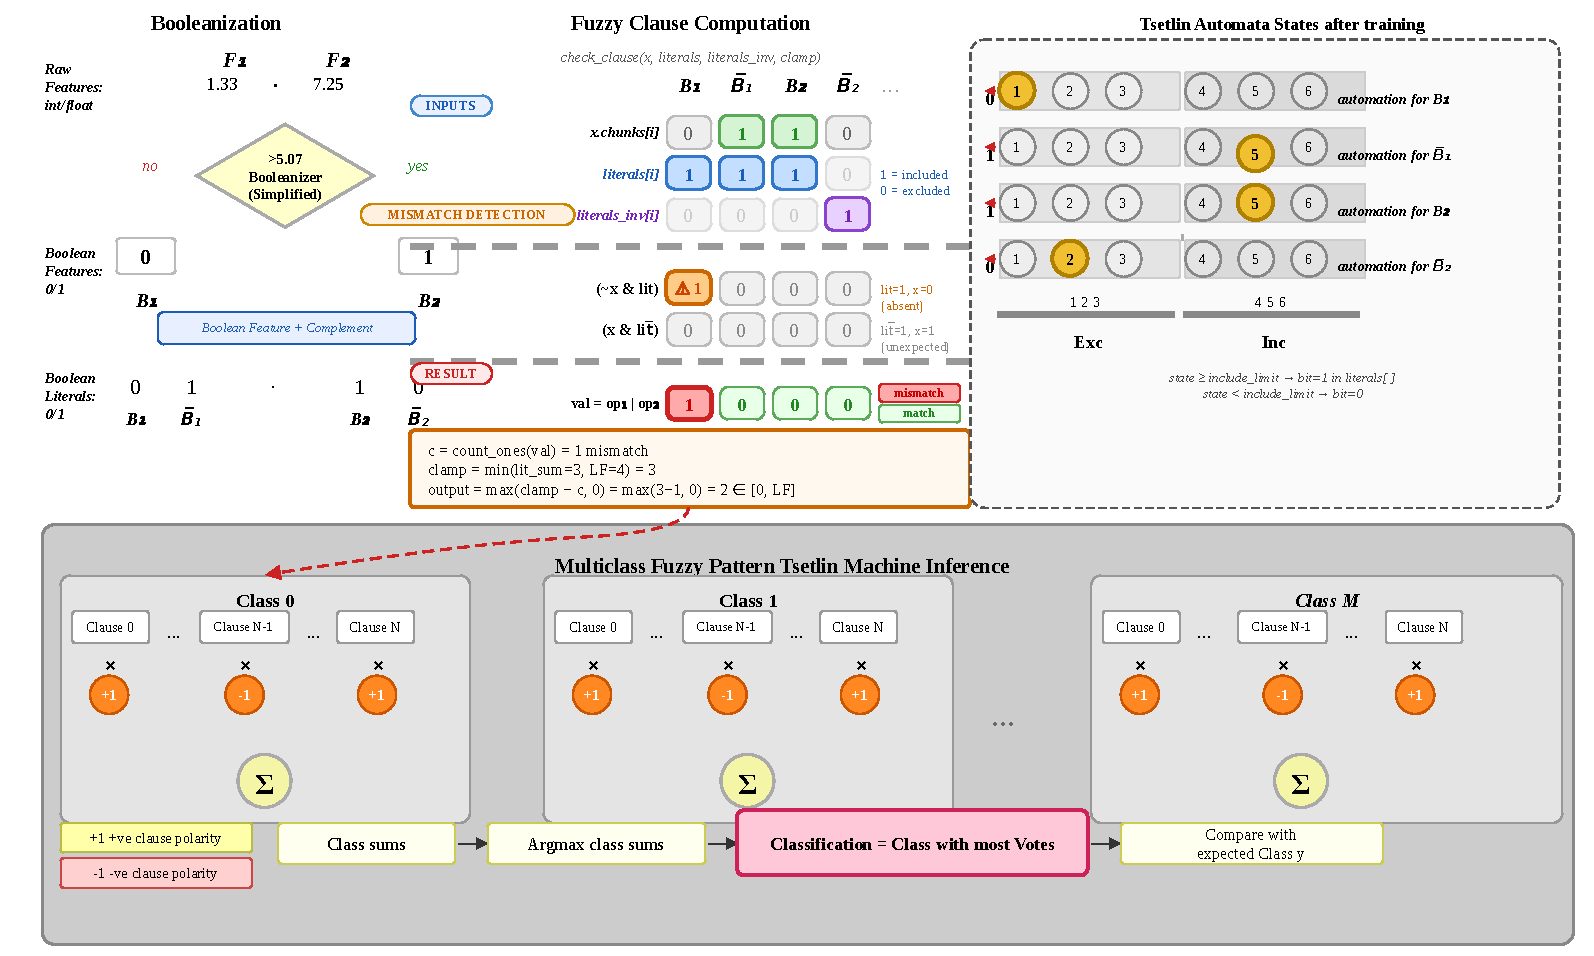
\includegraphics[width=2\columnwidth]{TII-Articles-LaTeX-template/Fptm1.pdf}
    \caption{Data flow of the Fuzzy-Pattern Tsetlin Machine: binarised
    input features are read by teams of Tsetlin automata that fix the
    literals of each clause, the clauses produce graded outputs, and
    the per-class signed vote totals yield the prediction.}
    \label{fig:tm-architecture}
\end{figure*}

\section{Experimental Setup}
\label{sec:experiments}

\subsection{Datasets}
\label{sec:datasets}

Four publicly available benchmarks are used in the evaluation. They
were selected to represent both conventional IoT network traffic and
IoMT traffic, and to cover differences in
scale, feature representation, and attack taxonomy. Their main
characteristics are summarised in
Table~\ref{tab:datasets_transposed}.
Record and feature counts correspond to the original datasets prior to
preprocessing, whereas training and testing splits follow the unified
pipeline described in Section~\ref{sec:preprocessing}.

\textbf{NSL-KDD}~\cite{tavallaee2009nslkdd} is a widely used benchmark
for network intrusion detection. It was introduced to address the
limitations of the KDD CUP 99 dataset, particularly redundancy and
class imbalance. The dataset contains 41 handcrafted features derived
from TCP/IP connections, and traffic is grouped into five classes:
Normal, DoS, Probe, R2L, and U2R.

\textbf{TON\_IoT}~\cite{moustafa2021toniot} represents IoT/IIoT
environments with heterogeneous traffic collected from a distributed
testbed comprising cloud, edge, and IoT layers. It includes ten attack
categories such as DoS, DDoS, ransomware, and MITM. The dataset provides
44 features capturing protocol, statistical, and payload-level
characteristics.

\textbf{MedSec-25}~\cite{medsec25} is a recent IoMT dataset derived from
a simulated healthcare environment with interconnected medical devices.
It consists of 78 features and five classes (Normal, DoS, DDoS, MITM,
and Reconnaissance), with a total of 554,534 samples. Its rich feature
space and scale make it suitable for assessing IoMT-oriented
intrusion-detection models.

\textbf{WUSTL-EHMS-2020}~\cite{hady2020wustl} combines network traffic
features with physiological signals collected from wearable medical
devices in a real healthcare monitoring system. It includes three
classes (Normal, Spoofing, and Data Alteration) and 44 features. This hybrid
dataset enables evaluation of models that combine cyber and physical
context for intrusion detection.

\begin{table*}[t]
\caption{Summary of IoT and IoMT intrusion detection datasets used in this study.}
\label{tab:datasets_transposed}
\centering
\renewcommand{\arraystretch}{1.2}
\small
\begin{tabular}{@{}lcccc@{}}
\toprule
\textbf{Attribute} & \textbf{NSL-KDD} & \textbf{TON\_IoT} & \textbf{MedSec-25} & \textbf{WUSTL-EHMS-2020} \\
\midrule
Records   & 148,517 & 211,043 & 554,534 & 16,318 \\
Features  & 41      & 44      & 78      & 44 \\
Classes   & 5       & 10      & 5       & 3 \\
Domain    & IoT network flow & IoT multi-protocol & IoMT network flow & IoMT (network + biomedical) \\
Train     & 118,813 & 168,834 & 443,627 & 13,054 \\
Test      & 29,704  & 42,209  & 110,907 & 3,264 \\
\bottomrule
\end{tabular}
\end{table*}

\subsection{Data Preprocessing}
\label{sec:preprocessing}

A unified preprocessing pipeline is applied across all datasets and
models to maintain comparability. Raw features are first loaded, and
class labels are encoded numerically. Non-informative attributes, such
as identifiers, are removed, and categorical features are transformed
using one-hot encoding where applicable. The data is then divided into
training and testing sets by a stratified 80/20 split to preserve class
distributions. Infinite values are replaced with missing values, and
missing entries are imputed using medians computed from the training
set only. Constant features are eliminated according to zero variance in
the training data. Highly correlated features are then removed using a
threshold of $|r| > 0.99$, also determined exclusively from the
training set.

\subsection{FPTM Configuration}
\label{sec:fptm-config}

The Fuzzy Pattern Tsetlin Machine (FPTM) is configured using
dataset-specific hyperparameters obtained through tuning.
The model is parameterised by $C$ (number of clauses per class per
polarity), $T$ (voting target), $s$ (specificity), $L$ (maximum number
of literals per clause), $L_f$ (fuzzy clamp threshold), and $E$
(training epochs).

All experiments employ the proposed GLADE binariser with a fixed
discretisation parameter of $n_{\text{bins}} = 15$ across all datasets.

The hyperparameters are selected via a grid search over the
configuration space for each dataset, subject to the constraint that
$C \leq 100$ and $C$ is an even number. The final configurations are
reported in Table~\ref{tab:tm_hparams}.

\begin{table}[t]
\centering
\caption{Tuned FPTM hyperparameters per dataset.}
\label{tab:tm_hparams}
\renewcommand{\arraystretch}{1.2}
\small
\begin{tabular}{|l|c|c|c|c|c|c|}
\hline
\textbf{Dataset} & $C$ & $T$ & $s$ & $L$ & $L_f$ & $E$ \\
\hline
NSL-KDD         & 90  & 12 & 200 & 40 & 8  & 80  \\
\hline
TON\_IoT        & 100 & 15 & 20  & 25 & 8  & 200 \\
\hline
MedSec-25       & 80  & 12 & 75  & 30 & 8  & 300 \\
\hline
WUSTL-EHMS-2020 & 60  & 8  & 300 & 50 & 15 & 200 \\
\hline
\end{tabular}
\end{table}

\subsection{Baselines}
\label{sec:baselines}

The baseline set comprises standard machine-learning classifiers with
library-default configurations, together with variants whose capacity
is aligned with the tuned FPTM. The default baselines include XGBoost,
Random Forest, Logistic Regression, Linear SVM, Gaussian Naive Bayes
(reported as NaiveBayes), and $k$-Nearest Neighbours ($k=5$).

For a second comparison point, additional variants are constructed by
matching model capacity to the FPTM configuration. For tree ensembles,
the number of estimators is set to the clause count $C$. The matched
variants are denoted with the suffix \texttt{\_Cmatched}. All models
are implemented using scikit-learn~\cite{pedregosa2011scikit} and the
official XGBoost Python package; the full set of baseline
configurations is listed in
Table~\ref{tab:model_configs}.
\begin{table}[t]
\centering
\caption{Baseline model configurations. Starred ($^\ast$) models have
capacity matched to the FPTM clause count $C$.}
\label{tab:model_configs}
\renewcommand{\arraystretch}{1.2}
\small
\begin{tabular}{@{}p{0.34\columnwidth}p{0.58\columnwidth}@{}}
\toprule
\textbf{Model} & \textbf{Configuration} \\
\midrule
\multicolumn{2}{@{}l}{\textit{Default baselines}} \\
XGBoost            & n=100, max depth=6, learning rate=0.1 \\
Random Forest      & n=100, max depth=none \\
k-NN ($k=5$)       & uniform weights, Minkowski distance \\
Logistic Regression & L2 regularisation, $C=1.0$, LBFGS \\
Linear SVM         & $C=1.0$, squared hinge loss \\
Naive Bayes        & GaussianNB \\
\midrule
\multicolumn{2}{@{}l}{\textit{FPTM-matched variants}} \\
XGBoost\_Cmatched$^\ast$      & n\_estimators = $C$, max depth = 6, learning rate = 0.1 \\
RandomForest\_Cmatched$^\ast$ & n\_estimators = $C$, max depth = none \\
\bottomrule
\end{tabular}
\end{table}

\section{Results}
\label{sec:results}

\subsection{Binariser Comparison}
\label{sec:res-binarisers}

Table~\ref{tab:binarizer_comparison} evaluates the impact of the
binarisation scheme while keeping the FPTM hyperparameters fixed.
Three approaches are compared: GLADE, the \texttt{StandardBinarizer}
from TMU, and a uniform thermometer encoder that places evenly spaced
thresholds within each feature range.

Across all datasets, GLADE produces the fewest binary features. Its
Boolean representation is reduced by roughly 20\%--50\% relative to the
\texttt{StandardBinarizer} and by roughly 30\%--85\% relative to the
thermometer encoder, with the largest contraction observed on the
higher-dimensional NSL-KDD feature space. Comparable classification
performance is retained despite this reduction. The difference is most
visible on TON\_IoT and MedSec-25, where sparse feature distributions
are less effectively captured by the alternative encoders. As shown in
Table~\ref{tab:binarizer_comparison}, GLADE yields the smallest
Boolean representations while preserving accuracy and macro-F1 scores
within the range required for the downstream detector.

\begin{table*}[t]
\centering
\renewcommand{\arraystretch}{1.2}
\small
\caption{Comparison of binarisation methods with $n_\text{bins}=15$.
Best values per dataset and metric are shown in \textbf{bold}.
GLADE+FPTM rows match those reported in Table~\ref{tab:results_part1}
and Table~\ref{tab:results_part2}.}
\label{tab:binarizer_comparison}
\resizebox{\textwidth}{!}{%
\begin{tabular}{|l|ccc|ccc|ccc|}
\hline
 & \multicolumn{3}{c|}{\textbf{GLADE}}
 & \multicolumn{3}{c|}{\textbf{\texttt{StandardBinarizer}}}
 & \multicolumn{3}{c|}{\textbf{Thermometer}} \\
\hline
\textbf{Dataset} & Bits & Acc & F1 & Bits & Acc & F1 & Bits & Acc & F1 \\
\hline
NSL-KDD         & \textbf{253} & \textbf{0.9951} & \textbf{0.9356} & 472 & 0.9941 & 0.9342 & 1652 & 0.9859 & 0.8846 \\
\hline
TON\_IoT        & \textbf{122} & \textbf{0.9708} & \textbf{0.9410} & 186 & 0.8416 & 0.7947 & 532  & 0.6404 & 0.5658 \\
\hline
MedSec-25       & \textbf{351} & \textbf{0.9706} & \textbf{0.8697} & 698 & 0.8830 & 0.7265 & 756  & 0.8463 & 0.5576 \\
\hline
WUSTL-EHMS-2020 & \textbf{256} & \textbf{0.9421} & \textbf{0.7868} & 313 & 0.9381 & 0.7388 & 378  & 0.9121 & 0.6146 \\
\hline
\end{tabular}
}
\end{table*}

\subsection{Main Classification Benchmark}
\label{sec:res-main}

Tables~\ref{tab:results_part1} and~\ref{tab:results_part2} report the
classification performance of the tuned GLADE+FPTM pipeline alongside
the baseline models across the four datasets. Results are presented in
terms of accuracy, macro F1, precision, recall, and serialized model
size. The inference-time column reports mean per-sample latency in
microseconds for the models included in the benchmark.

Across the four datasets, the GLADE+FPTM pipeline remains competitive
with the baseline methods while requiring a markedly smaller
deployment artifact. Its macro-F1 score is close to that of the
tree-based baselines on several datasets, whereas the serialized model
footprint is reduced by one to three orders of magnitude. On
WUSTL-EHMS-2020, the smallest and most variable dataset considered, a
balanced trade-off between accuracy, macro F1, and model size is
obtained.

\begin{table*}[t]
\centering
\caption{Classification results on NSL-KDD and TON\_IoT datasets.}
\label{tab:results_part1}
\resizebox{\textwidth}{!}{%
\begin{tabular}{llcccccc}
\hline
\textbf{Dataset} & \textbf{Model} & \textbf{Accuracy} & \textbf{Macro F1} & \textbf{Precision} & \textbf{Recall} & \textbf{Size (KB)} & \textbf{Inference ($\mu$s/sample)} \\
\hline

\multirow{9}{*}{NSL-KDD}
 & XGBoost                & 0.9956 & 0.9488 & 0.9442 & 0.9558 & 1266 & 9.988 \\
 & XGBoost\_Cmatched      & 0.9952 & 0.9429 & 0.9419 & 0.9458 & 1161 & 9.122 \\
 & GLADE+FPTM             & 0.9951 & 0.9356 & 0.9424 & 0.9294 & 51.1 & 3.387 \\
 & kNN\_5                 & 0.9894 & 0.8855 & 0.9052 & 0.8691 & 110463 & 4118.039 \\
 & LogisticRegression     & 0.9769 & 0.8580 & 0.8877 & 0.8337 & 8.6  & 1.420 \\
 & RandomForest           & 0.9926 & 0.8563 & 0.9647 & 0.8167 & 27239 & 12.697 \\
 & LinearSVM              & 0.9655 & 0.8530 & 0.8986 & 0.8194 & 8.6  & 1.393 \\
 & RandomForest\_Cmatched & 0.9625 & 0.5843 & 0.5821 & 0.5869 & 962  & 6.124 \\
 & NaiveBayes             & 0.7567 & 0.4423 & 0.5765 & 0.6726 & 13.2 & 4.652 \\
\hline

\multirow{9}{*}{TON\_IoT}
 & XGBoost                & 0.9775 & 0.9511 & 0.9439 & 0.9614 & 2508 & 22.125 \\
 & XGBoost\_Cmatched      & 0.9764 & 0.9498 & 0.9424 & 0.9608 & 1899 & 18.138 \\
 & RandomForest           & 0.9765 & 0.9467 & 0.9366 & 0.9637 & 62383 & 11.077 \\
 & kNN\_5                 & 0.9742 & 0.9441 & 0.9430 & 0.9461 & 51444 & 5225.119 \\
 & GLADE+FPTM             & 0.9708 & 0.9410 & 0.9322 & 0.9560 & 76.2 & 8.567 \\
 & RandomForest\_Cmatched & 0.8771 & 0.7814 & 0.7961 & 0.7798 & 841  & 11.299 \\
 & LogisticRegression     & 0.7076 & 0.6347 & 0.7154 & 0.6494 & 5.5  & 0.632 \\
 & LinearSVM              & 0.7114 & 0.6273 & 0.7106 & 0.6486 & 5.5  & 0.629 \\
 & NaiveBayes             & 0.3875 & 0.3269 & 0.3694 & 0.4201 & 8.5  & 3.161 \\
\hline
\end{tabular}
}
\end{table*}


\begin{table*}[t]
\centering
\caption{Classification results on MedSec-25 and WUSTL-EHMS-2020 datasets.}
\label{tab:results_part2}
\resizebox{\textwidth}{!}{%
\begin{tabular}{llcccccc}
\hline
\textbf{Dataset} & \textbf{Model} & \textbf{Accuracy} & \textbf{Macro F1} & \textbf{Precision} & \textbf{Recall} & \textbf{Size (KB)} & \textbf{Inference ($\mu$s/sample)} \\
\hline

\multirow{9}{*}{MedSec-25}
 & XGBoost                & 0.9768 & 0.8984 & 0.9005 & 0.9004 & 1701 & 12.091 \\
 & RandomForest           & 0.9767 & 0.8980 & 0.9022 & 0.9036 & 146062 & 7.521 \\
 & XGBoost\_Cmatched      & 0.9753 & 0.8926 & 0.8951 & 0.8951 & 939  & 8.273 \\
 & kNN\_5                 & 0.9733 & 0.8799 & 0.8752 & 0.8848 & 190624 & 15527.080 \\
 & GLADE+FPTM             & 0.9706 & 0.8697 & 0.8750 & 0.8752 & 41.5 & 5.471 \\
 & RandomForest\_Cmatched & 0.9611 & 0.8390 & 0.8631 & 0.8367 & 525  & 5.914 \\
 & LogisticRegression     & 0.9413 & 0.7763 & 0.7891 & 0.7853 & 4.8  & 0.901 \\
 & LinearSVM              & 0.8538 & 0.5146 & 0.6990 & 0.4660 & 4.7  & 0.823 \\
 & NaiveBayes             & 0.7673 & 0.4218 & 0.4803 & 0.5192 & 6.8  & 2.751 \\
\hline

\multirow{9}{*}{WUSTL-EHMS-2020}
 & GLADE+FPTM             & 0.9421 & 0.7868 & 0.8932 & 0.7559 & 25.2 & 1.446 \\
 & kNN\_5                 & 0.9375 & 0.7922 & 0.8445 & 0.7684 & 2857 & 364.308 \\
 & XGBoost                & 0.9406 & 0.7590 & 0.9151 & 0.7314 & 615  & 5.537 \\
 & XGBoost\_Cmatched      & 0.9354 & 0.7118 & 0.9198 & 0.6994 & 388  & -- \\
 & RandomForest           & 0.9320 & 0.6778 & 0.8910 & 0.6807 & 14385 & 4.380 \\
 & RandomForest\_Cmatched & 0.9305 & 0.6554 & 0.9671 & 0.6692 & 381  & -- \\
 & LinearSVM              & 0.9286 & 0.6449 & 0.6253 & 0.6657 & 2.4  & 0.122 \\
 & LogisticRegression     & 0.9280 & 0.6430 & 0.6220 & 0.6655 & 2.5  & 0.128 \\
 & NaiveBayes             & 0.1293 & 0.3643 & 0.6570 & 0.6668 & 3.0  & 0.511 \\
\hline
\end{tabular}
}
\end{table*}

\subsection{Serialization and Compression}
\label{sec:res-compression}

For deployment on resource-constrained edge devices, the trained
GLADE+FPTM pipeline is serialized into a single self-describing
container in which both the GLADE binarization thresholds and the FPTM
clause bitmasks are stored. Two equivalent formats containing
identical information are evaluated:

\begin{itemize}
    \item \textbf{\texttt{model.pkl}}: an uncompressed Python pickle
    file that stores the complete GLADE state (feature indices and
    thresholds) together with the TM rule representation, including
    the per-class positive and negative clause masks and their
    corresponding clamp values.

    \item \textbf{\texttt{model.fbz}}: the proposed
    \emph{Fuzzy-Bitmask Zstd (FBZ)} container, a compact binary format
    introduced in this work for deployment-oriented storage of the
    GLADE+FPTM inference artifact. The FBZ file consists of a fixed
    12-byte header followed by a Zstandard-compressed payload
    (zstd level~1). The header encodes the magic identifier, format
    version, compression level, dimensionality parameters
    (\texttt{n\_bits} and \texttt{n\_classes}), and the global clamp
    cap. Decoding requires only a standard zstd decompressor and
    little-endian integer unpacking, which supports portability across
    lightweight runtimes implemented in C, Rust, Go, or JavaScript.
\end{itemize}

Fig.~\ref{fig:storage_bar} compares the on-disk storage requirements
of the two formats. Across all four datasets, the FBZ container
reduces the deployable model footprint to approximately
21--30\% of the uncompressed pickle size. Specifically, the model
size is reduced from $25.2$\,KB to $7.1$\,KB on WUSTL-EHMS-2020,
from $51.1$\,KB to $13.7$\,KB on NSL-KDD, from $76.2$\,KB to
$16.2$\,KB on TON\_IoT, and from $41.5$\,KB to $12.3$\,KB on
MedSec-25. The compression process is strictly lossless, and exact
prediction equivalence after serialization and deserialization was
verified on the test split of every dataset.

\begin{figure}[t]
\centering
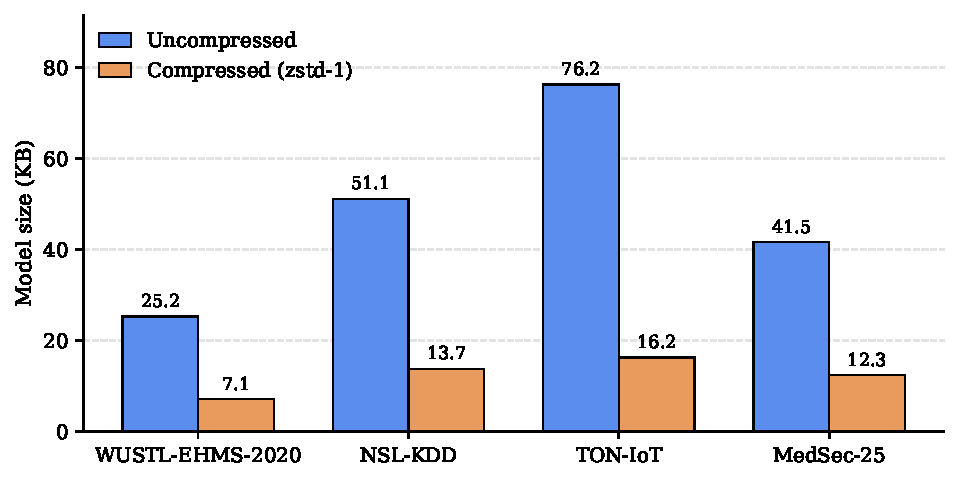
\includegraphics[width=\columnwidth]{figures/fig_storage_bar.pdf}
\caption{Storage footprint of the GLADE+FPTM model using
uncompressed (\texttt{model.pkl}) and compressed
(\texttt{model.fbz}) formats. Lower is better.}
\label{fig:storage_bar}
\end{figure}
\subsection{Compression Method Comparison}
\label{sec:res-codecs}

To position zstd-1 within the broader compression design space, the
uncompressed FBZ payload for each dataset is evaluated across
codec families and levels using the codec sweep benchmark
(\texttt{bench\_codecs\_sweep.py} $\rightarrow$
\texttt{SUMMARY\_codecs\_sweep.json}). The canonical payload contains
the GLADE thresholds and TM clause bitmasks with the FBZ header
stripped and the codec field set to 0 (uncompressed). Raw sizes are
approximately 31.3\,KB (NSL-KDD), 33.3\,KB (TON\_IoT), 38.5\,KB
(MedSec-25), and 13.8\,KB (WUSTL-EHMS-2020). Each payload is
round-tripped through all levels of five lossless codec families:
Zstandard (1--22), gzip (DEFLATE, 1--9), LZMA2 (0--9), Brotli (0--11),
and bzip2 (1--9). All compression and decompression operations are run
in memory on byte arrays, so timings reflect the codec only. Each
value is reported as the mean over 200 iterations (20 for the very-slow
settings), and every round-trip is verified byte-exact. For each
family, level, and dataset the benchmark records compressed size,
compression ratio (raw $\div$ compressed), compression time, and
decompression time. The size is the compressed byte count and thus
the exact on-disk size of the \texttt{.fbz} file.

Figures~\ref{fig:codec_size}--\ref{fig:codec_decomp} show the sweep
curves for TON\_IoT, which has the largest payload. To keep the linear
axes readable, the highest-effort settings are excluded from the plots:
Zstandard levels 1--10, gzip levels 1--7, LZMA2 levels 0--6, and
Brotli levels 0--8 are shown. bzip2 is omitted because its level
parameter does not affect this payload size and because it is less
favorable on the measured metrics. Zstandard is drawn in bold, and the
default setting (zstd-1) is marked with a gold star.

Three metrics are evaluated for each codec--dataset pair:
compressed size (Fig.~\ref{fig:codec_size}), compression time
(Fig.~\ref{fig:codec_comp}), and decompression time
(Fig.~\ref{fig:codec_decomp}). The results indicate the following:

\begin{enumerate}
    \item \textbf{Compressed size:} For TON\_IoT, zstd-1 already
    reduces the model to 16.2\,KB (2.05$\times$). Pushing any family
    to its high-effort end yields only marginal additional savings
    (approximately 0.5--0.9\,KB). gzip remains the largest at
    17.0--18.8\,KB, while LZMA2 reaches 16.2\,KB only from preset 4
    upward.

    \item \textbf{Compression time:} zstd has the lowest cost at every
    level, with zstd-1 at approximately 0.08\,ms versus gzip-1 at
    0.61\,ms and LZMA2 at 2.2\,ms minimum; both gzip and LZMA2 climb
    to 4--8\,ms at higher presets.

    \item \textbf{Decompression time:} Times are roughly constant
    within each family. zstd reaches approximately 0.03\,ms, Brotli
    about 0.12\,ms
    ($\sim$4$\times$), gzip about 0.19\,ms ($\sim$6$\times$), and
    LZMA2 about 0.8\,ms ($\sim$27$\times$). This property is relevant
    for edge deployment where decompression occurs at load time.
\end{enumerate}

Based on these results, zstd-1 is selected as the default FBZ codec
because it lies near the knee of the size--latency trade-off. Higher
levels or alternative codecs provide only marginal size reductions for
this payload while increasing compression or decompression time.

\begin{figure}[t]
\centering
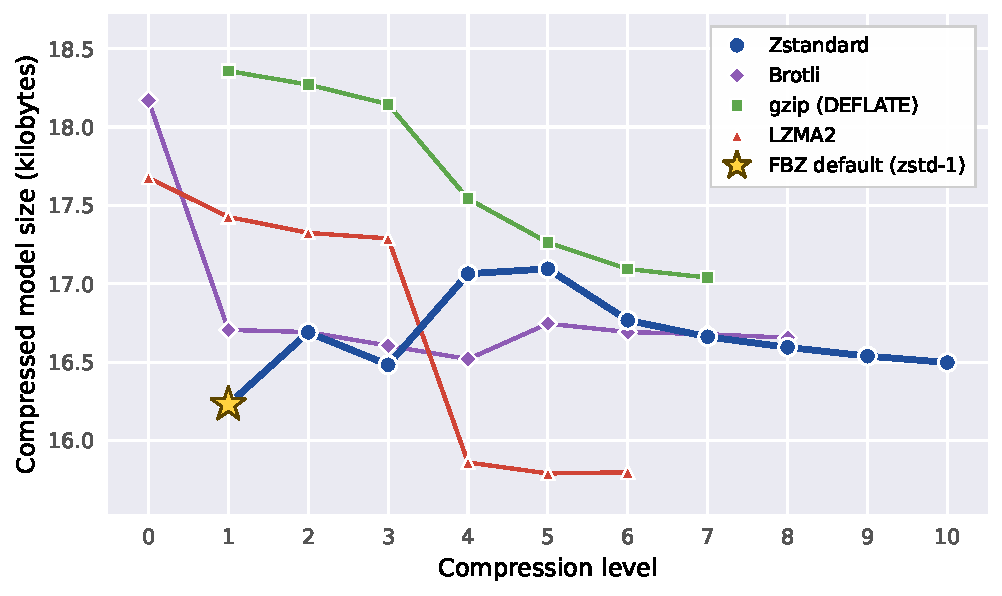
\includegraphics[width=\columnwidth]{figures/fig_codec_size_sweep.pdf}
\caption{Compression ratio achieved by different lossless codecs
for the serialized GLADE+FPTM model. Higher values indicate greater
compression efficiency.}
\label{fig:codec_size}
\end{figure}

\begin{figure}[t]
\centering
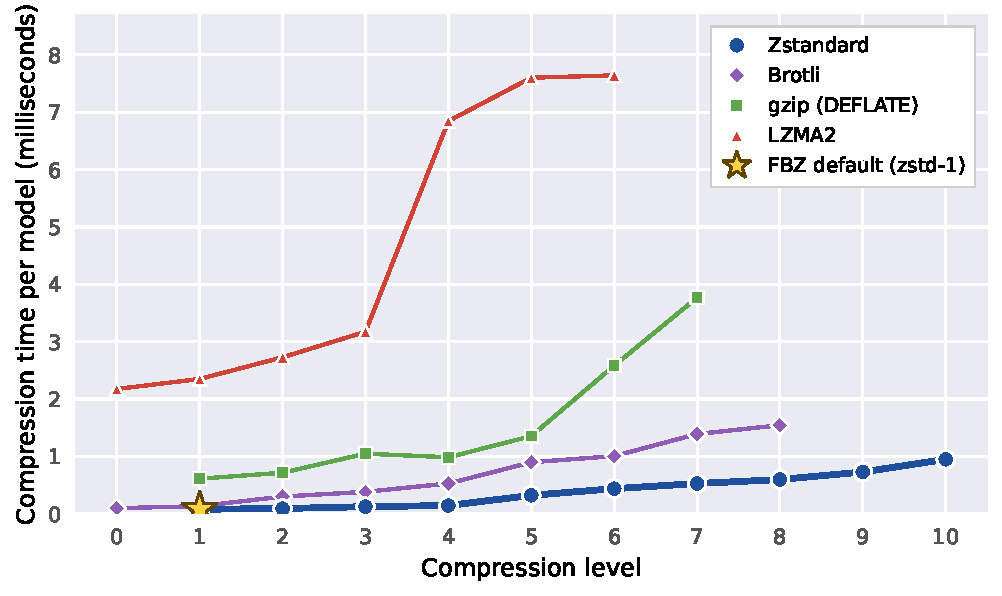
\includegraphics[width=\columnwidth]{figures/fig_codec_comp_sweep.pdf}
\caption{Compression latency of the evaluated codecs measured using
in-memory \texttt{BytesIO} buffers. Lower values indicate faster
compression.}
\label{fig:codec_comp}
\end{figure}

\begin{figure}[t]
\centering
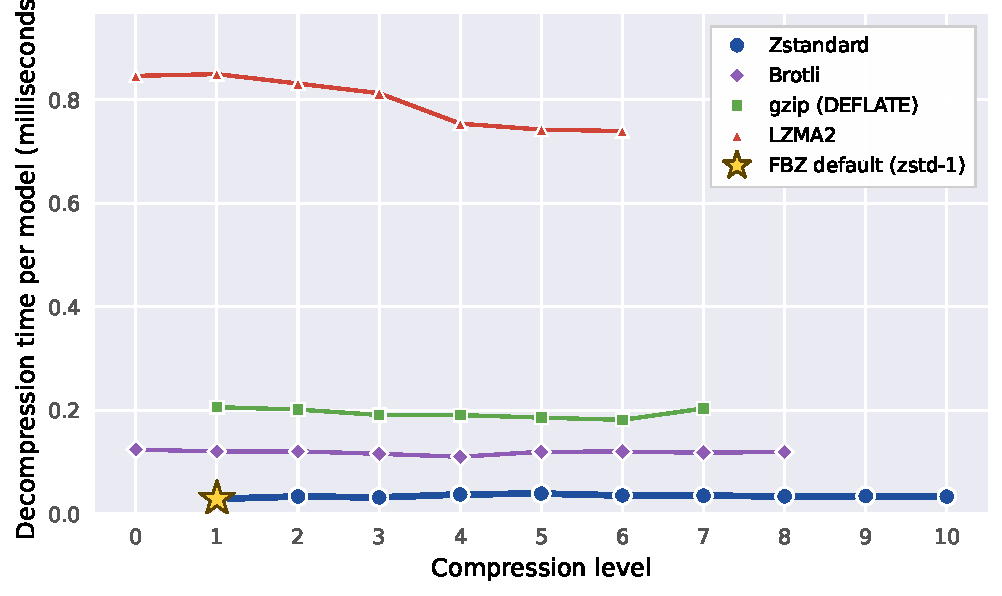
\includegraphics[width=\columnwidth]{figures/fig_codec_decomp_sweep.pdf}
\caption{Decompression latency of the evaluated codecs under the
same experimental setup as Fig.~\ref{fig:codec_comp}. Lower values
indicate faster decompression.}
\label{fig:codec_decomp}
\end{figure}

\subsection{Edge Deployment: Binarisation Latency on Raspberry Pi 5}
\label{sec:res-edge}

To assess real-time feasibility on resource-constrained hardware, the
GLADE binarisation step is timed against the TMU
\texttt{StandardBinarizer} and a conventional thermometer encoder on a
Raspberry~Pi~5 using the NEON SIMD path. Two execution modes are
reported in Fig.~\ref{fig:edge_latency}. In the element-wise transform,
one Boolean value is emitted for each generated literal. This mode is
useful for isolating the cost of threshold evaluation and for comparing
different binarisers before the classifier representation is imposed. In
the bit-packed transform, the Boolean literals are written directly into
64-bit words, which is the format consumed by the FPTM clause kernels.
This mode therefore reflects the deployable preprocessing path used
before bitwise clause evaluation. All values are mean per-sample
latencies in microseconds.

\begin{figure*}[!t]
\centering
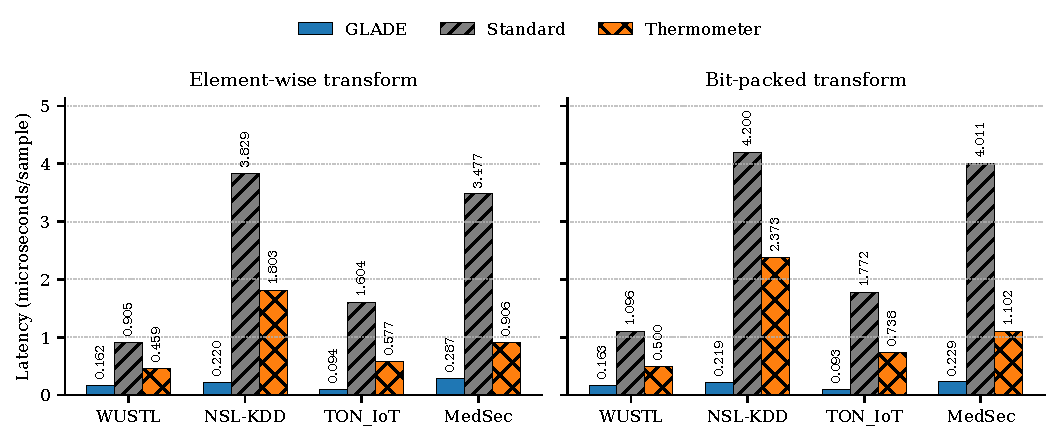
\includegraphics[width=0.92\textwidth]{figures/fig_edge_binarization_latency.pdf}
\caption{Raspberry~Pi~5 binarisation latency for GLADE,
\texttt{StandardBinarizer}, and thermometer encoding using element-wise
and bit-packed transforms. The y-axis is linear, and lower values
indicate lower per-sample preprocessing latency.}
\label{fig:edge_latency}
\end{figure*}

On the Raspberry~Pi~5, GLADE binarisation completes in well under one
microsecond per sample on every dataset. Relative to the
\texttt{StandardBinarizer}, latency is reduced by
$5.59\times$--$19.18\times$, with the largest gains observed on the
higher-dimensional NSL-KDD and TON\_IoT feature spaces. Relative to
thermometer encoding, the measured reduction reaches $10.84\times$.
The same pattern is preserved in bit-packed mode, indicating that the
compact Boolean representation produced by GLADE can be converted into
lower preprocessing latency on embedded hardware.


\section{Conclusion}
\label{sec:conclusion}

This paper has presented GLADE, a gap-aware lightweight adaptive
discretisation engine for transforming heterogeneous IoT feature
streams into compact Boolean representations, together with its
integration with the Fuzzy Pattern Tsetlin Machine (FPTM) for
resource-constrained intrusion detection. The resulting pipeline has
been positioned as a viable alternative when deployment constraints
limit the practicality of conventional machine-learning detectors, and
as a component that may coexist with such detectors in hybrid security
architectures. On NSL-KDD, TON\_IoT, MedSec-25, and WUSTL-EHMS-2020,
the Boolean feature space was reduced by 30\%--85\% relative to
thermometer encoding while competitive accuracy and macro-F1
scores were retained. Serialized model sizes as low as 7.1\,KB were
obtained, and Raspberry~Pi~5 measurements showed binarisation latency
reductions of up to $19\times$ relative to the standard binariser and
up to $11\times$ relative to thermometer encoding. The results indicate
that GLADE+FPTM is a practical option for IoT intrusion-detection
deployments in which transparent rule logic, compact storage, and
bitwise execution are required.

\bibliographystyle{IEEEtran}
\bibliography{references}

\end{document}
